\documentclass[a4paper,12pt]{article}
\usepackage[french]{babel}
\usepackage[T1]{fontenc}
\usepackage[utf8]{inputenc}
\usepackage{graphicx}
\usepackage{pdfpages}
\usepackage{svg}

\title{Capteur - Compte rendu TP capteurs de température}
\author{
	Thibault THEOLOGIEN - Florian MARTIN - Youssef ZERHOUNI\\
	INSA Rouen\\
	ASI 3.2 - Groupe 1.1
}

\begin{document}
	\maketitle
	\tableofcontents
	\newpage

  \par Le but de ce TP était de nous familiariser avec trois différents capteurs de température: une sonde à platine PT100, un thermocouple et une thermistance à pente négative (NTC).

  \section{Capteur PT100}

    \subsection{Réglage de la compensation}
      \par Tout d'abord on commence par mettre les cavaliers dans le bon endroit de la manière suivante :
      \begin{itemize}
        \item JP1 = On
        \item JP2 = On
        \item JP3 = Off
      \end{itemize}
      Ensuite on règle le potentiomètre de compensation afin d'avoir une valeur de sortie de 0V en température ambiante.

    \subsection{Réglage du gain}
      \par Maintenant que la compensation est correctement réglée, il est temps de nous occuper du gain.\\
      Pour cela il faut changer l'emplacement des cavaliers de la manière suivante :
      \begin{itemize}
        \item JP1 = On
        \item JP2 = Off
        \item JP3 = On
      \end{itemize}
      Ensuite on règle le potentiomètre de gain pour obtenir une sortie qui correspond à la température ambiante.
      Dans notre cas on choisi une sortie à 2,6 volts, en admettant que la température ambiante est dans les environ de 25\degre.

    \subsection{Mesures}
      \par Une fois les réglages terminés on passe en mode mesure en laissant les cavaliers dans leur position précédente.\\
      On fait trois mesures correspondant à trois températures différentes:
      \begin{itemize}
        \item Corps humain: 3.51 V
        \item Glace: 0.63 V
        \item Ambiance: 2.64 V
      \end{itemize}

    \subsection{Simulation}
      \par On fait une simulation des températures qu'on devrait obtenir en utilisant différentes valeurs de résistance à la place de la PT100.
			On obtient le tableau de données suivant:

      \par Ces données nous permettent de tracer les courbes suivantes, comparant les valeurs de température théorique et celle fourni par la documentation de la PT100 :
			\begin{center}
				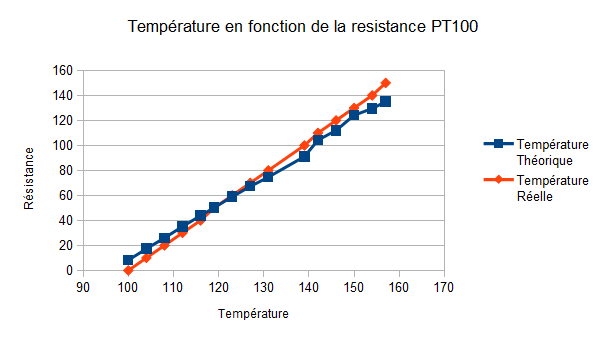
\includegraphics[width=12cm]{../Images/GraphPT100.png}
			\end{center}
    \newpage

  \section{Capteur de type NTC}
		\subsection{Simulation}
			\par On fait une simulation des températures qu'on devrait obtenir en utilisant différentes valeurs de résistance à la place de la PT100.
			On obtient le tableau de données suivant:

			\par Ces données nous permettent de tracer les courbes suivantes, comparant les valeurs de température théorique et celle fourni par la documentation de la PT100 :
			\begin{center}
				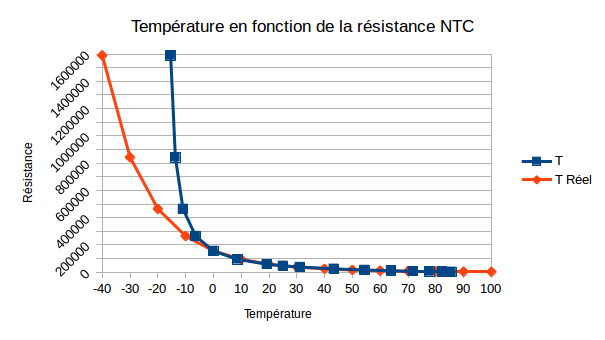
\includegraphics[width=12cm]{../Images/GraphNTC.png}
			\end{center}

\end{document}
